\documentclass{svproc}

\usepackage{url}
\usepackage{bm}
\usepackage{amsmath}
\usepackage{microtype}
\usepackage{hyphenat}
\usepackage{tabularx}
\usepackage{tikz}
\usetikzlibrary{arrows.meta,positioning,fit,backgrounds,calc}
\usepackage{graphicx}
\usepackage{bytefield}
\usepackage{pgfplots}
\pgfplotsset{compat=1.18}
\usepackage{algorithm}
\usepackage{algpseudocode}
\usepackage{listings}
\lstset{
  basicstyle=\ttfamily\scriptsize,
  keywordstyle=\bfseries,
  columns=fullflexible,
  showstringspaces=false,
  frame=single,
  framerule=0.4pt,
  xleftmargin=4pt,
  aboveskip=6pt, belowskip=6pt,
  numbers=none,
  breaklines=true,
}

\def\UrlFont{\rmfamily}

\begin{document}
\mainmatter

\title{GenoID: A Declarative Framework for Structured RFC 9562 v8 UUIDs via Constraint-Guided Repair}

\titlerunning{GenoID: Declarative Structured RFC 9562 v8 UUIDs}

\author{Padala Manohar Maharshi\inst{1} \and Ouku Jasmine\inst{2}}

\authorrunning{Manohar and Jasmine}

\tocauthor{Padala Manohar Maharshi and Ouku Jasmine}
\institute{Vignan's Institute Of Information Technology, Vishakhapatnam, India\\
\email{pmmaharshi@vignaniit.edu.in} \textnormal{(ORCID: 0009-0006-5807-4151)},\\
\and
Vignan's Institute Of Information Technology, Vishakhapatnam, India \\ \email{oukujasmine@gmail.com}}

\maketitle              % typeset the title of the contribution

\begin{abstract}
Standard UUID generators cannot embed application-defined structure (a shard, a tenant, or a monotonic counter) inside a standards-compliant identifier without paying rejection sampling's exponential cost. RFC 9562 makes this gap explicit: version 8 reserves 122 bits for exactly this purpose but defines no algorithm to fill them. We close this gap with GenoID, a declarative composition framework that produces valid v8 UUIDs from arbitrary constrained fields at $O(k)$ cost, against rejection sampling's $O(64^k)$ worst case, verified across 100M identifiers with zero collisions and a full NIST SP 800-22 and dieharder statistical pass. The result is a portable algorithm, verified byte-identical across an independent Rust reimplementation, backed by formal complexity and entropy-preservation proofs and an explicit adversarial security analysis that separates GenoID's architectural contribution from the CSPRNG-inherited randomness quality beneath it. By making shard, tenant, and sequence identity a declarative property of the key itself, GenoID targets the data-systems layer directly.
\keywords{distributed data systems, sharding, UUID, RFC 9562}
\end{abstract}

\section{Introduction}

Imagine ten database servers where each record's ID must reveal which one owns it. RFC~9562's v8 UUID reserves 122 bits for application-defined structure but specifies no algorithm to fill them. GenoID is that missing algorithm: instead of rejection sampling's $O(64^k)$ draws, it produces correct keys on the first try in $O(k)$ work.

Existing UUIDs fall short: v4 carries no structure, v7 fixes one timestamp layout, and \texttt{pg\_uuid\_v8} embeds an encrypted timestamp with no multi-field composition. GenoID declares field structure once as a \texttt{V8Layout} and satisfies it by deterministic repair, drawing from pre-populated CSPRNG pools to amortize entropy cost.

\noindent\textbf{Contributions.}
\begin{itemize}
    \item A declarative RFC~9562 v8 layout abstraction for typed, constrained fields.
    \item A pooled generation architecture that amortizes CSPRNG draws, with a formal proof and empirical ablation showing pooling and composition are entropy-neutral on random-type fields.
    \item Constraint-guided repair: $O(k)$ per UUID vs $O(64^k)$ rejection sampling.
    \item An adversarial security analysis disclosing the bounded forward-secrecy window and by-design metadata leakage of structured layouts.
    \item Validation across collision-freedom at 100M scale, NIST and dieharder batteries, and multi-runtime throughput benchmarks, with limitations disclosed openly.
\end{itemize}

\section{Design}
\label{sec:design}
Think of a UUID's 122 free bits as a form with labeled blanks: timestamp, shard from a small set, monotonic counter. GenoID lets a developer declare that form once and fills every blank correctly on every call.

\medskip
\noindent\emph{Example:} a \texttt{dbkey} UUID for shard~3 at time~$t$: the first 48 bits read as $t$, the shard byte reads 3, a router extracts ``shard~3'' directly from the key. Remaining bits are random.

\subsection{Declarative layout}
\label{sec:layout}
A \texttt{V8Layout} declares ordered \texttt{V8Field}s with bit offset, length, type, and optional constraint.

\begin{lstlisting}[language=Java,
  caption={The \texttt{dbkey} layout declaration. Bit ranges 48--51
           (\texttt{ver}) and 64--65 (\texttt{var}) are never declared:
           \texttt{completeLayout} reserves them per RFC~9562 and fills
           every remaining undeclared range with random filler.},
  label={lst:dbkey}]
const dbkey: V8Layout = {
  name: "dbkey",
  fields: [
    { name: "timestamp", offset:  0, length: 48,
      type: "timestamp-ms" },
    { name: "shard",     offset: 52, length:  8,
      type: "shard",
      constraint: { kind: "allowed", allowed: [1,2,3,4,5] } },
    { name: "counter",   offset: 66, length: 16,
      type: "counter",
      constraint: { kind: "monotonic" } },
  ],
};
\end{lstlisting}

Listing~\ref{lst:dbkey} is the complete specification: no generation code is written per layout, and the same \texttt{repairConstraints} pass (Algorithm~\ref{alg:repair}) serves every declaration. Substituting \texttt{allowed: [1..5]} with a 12-bit tenant enum and an 8-bit region enum yields the \texttt{multitenant} layout without touching the generator.

\begin{figure}[!ht]
\centering
\resizebox{\columnwidth}{!}{%
\begin{bytefield}[bitwidth=1.05em,boxformatting={\centering\footnotesize}]{32}
  \bitbox{32}{\texttt{timestamp} (bits 0--31)} \\
  \bitbox{16}{\texttt{timestamp} 32--47}
    \bitbox{4}{\scriptsize ver$^\dagger$}
    \bitbox{8}{\texttt{shard}}
    \bitbox{4}{\scriptsize rnd} \\
  \bitbox{2}{\scriptsize var$^\dagger$}
    \bitbox{16}{\texttt{counter}}
    \bitbox{14}{random} \\
  \bitbox{32}{random}
\end{bytefield}%
}
\caption{RFC~9562 v8 UUID under the \texttt{dbkey} layout as four consecutive
32-bit words. $^\dagger$RFC-fixed: \texttt{ver} (bits 48--51), \texttt{var} (bits 64--65). All other bits carry the declared \texttt{timestamp}, \texttt{shard}, and \texttt{counter}; undeclared bits are random.}
\label{fig:layout}
\end{figure}

\subsection{Implementation: pooled two-parent assembly}
\label{sec:crossover}
Generation begins by populating two independent CSPRNG pools in full. A child UUID is then assembled field by field: one bit of an independently drawn \texttt{fieldSelect} chooses whether the child inherits from parent A or parent B (Fig.~\ref{fig:pipeline}). Because every field in both parents is independently CSPRNG-populated, and the select bit is independent of field contents, crossover\footnote{``Crossover'' and ``mutation'' are used as vocabulary for composition and repair, not optimization: GenoID has no fitness function, selective pressure, or generational loop.} never mixes partial values within a field.

\subsection{Constraint-guided repair}
\label{sec:repair}

\begin{algorithm}[!ht]
\caption{\texttt{repairConstraints}: single-pass constraint satisfaction}
\label{alg:repair}
\begin{algorithmic}[1]
\Require Layout $L$ with fields $f_1..f_n$; candidate 128-bit value $u$;
         monotonic state $M$
\Ensure  $u'$ satisfying every constraint declared in $L$
\For{each $f \in L.\textit{fields}$ with $f.\textit{constraint} \neq \textsc{null}$}
  \State $v \gets \textsc{ExtractBits}(u,\, f.\textit{offset},\, f.\textit{length})$
  \State $c \gets f.\textit{constraint}$
  \If{$c.\textit{kind} = \textsc{allowed}$}
    \State $v' \gets \arg\min_{a \in c.\textit{allowed}}
            \textsc{Hamming}(v, a)$
            \Comment{$O(|c.\textit{allowed}| \cdot f.\textit{length})$}
  \ElsIf{$c.\textit{kind} = \textsc{range}$}
    \State $v' \gets \min(\max(v,\, c.\textit{min}),\, c.\textit{max})$
            \Comment{$O(1)$}
  \ElsIf{$c.\textit{kind} = \textsc{monotonic}$}
    \State $v' \gets \max(v,\, M[f.\textit{name}])$;\;
           $M[f.\textit{name}] \gets v'$
            \Comment{$O(1)$}
  \EndIf
  \State $u \gets \textsc{WriteBits}(u,\, f.\textit{offset},\,
          f.\textit{length},\, v')$
\EndFor
\State \Return \textsc{SetVersionVariant}(u)
        \Comment{RFC~9562 \S4.2}
\end{algorithmic}
\end{algorithm}

Every branch assigns $v'$ unconditionally, so the loop body cannot fail and the procedure contains no backward jump: it executes exactly $k$ iterations for $k$ constrained fields, independent of the drawn value. Correctness is by construction: each branch's codomain is the constraint's satisfying set: 0 violations, not ``near 0.''

\begin{figure}[!ht]
\centering
\resizebox{\columnwidth}{!}{%
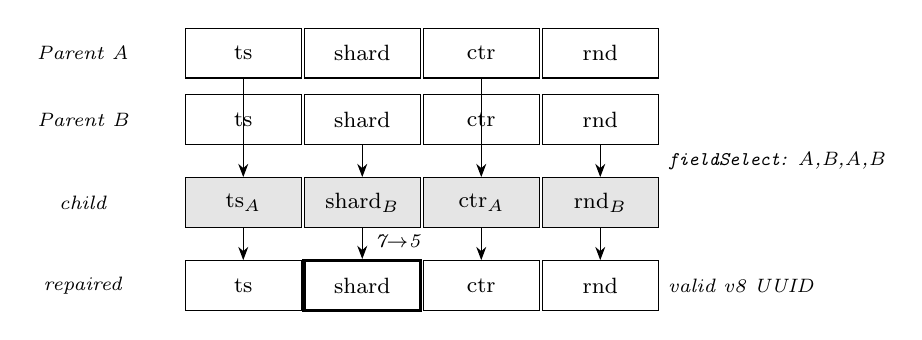
\begin{tikzpicture}[
  font=\footnotesize,
  cell/.style={draw,minimum width=42pt,minimum height=18pt,align=center},
  pick/.style={fill=black!10},
  lbl/.style={font=\scriptsize\itshape},
  >={Stealth[]}]
% Parent A
\node[lbl] at (-58pt,0) {Parent A};
\node[cell] (a1) at (0,0)    {ts};
\node[cell] (a2) at (43pt,0) {shard};
\node[cell] (a3) at (86pt,0) {ctr};
\node[cell] (a4) at (129pt,0){rnd};
% Parent B
\node[lbl] at (-58pt,-24pt) {Parent B};
\node[cell] (b1) at (0,-24pt)    {ts};
\node[cell] (b2) at (43pt,-24pt) {shard};
\node[cell] (b3) at (86pt,-24pt) {ctr};
\node[cell] (b4) at (129pt,-24pt){rnd};
% Child (fieldSelect: A,B,A,B)
\node[lbl] at (-58pt,-54pt) {child};
\node[cell,pick] (c1) at (0,-54pt)    {ts$_A$};
\node[cell,pick] (c2) at (43pt,-54pt) {shard$_B$};
\node[cell,pick] (c3) at (86pt,-54pt) {ctr$_A$};
\node[cell,pick] (c4) at (129pt,-54pt){rnd$_B$};
% select arrows
\draw[->] (a1) -- (c1); \draw[->] (b2) -- (c2);
\draw[->] (a3) -- (c3); \draw[->] (b4) -- (c4);
\node[lbl,right] at (150pt,-39pt) {\texttt{fieldSelect}: A,B,A,B};
% repair
\node[lbl] at (-58pt,-84pt) {repaired};
\node[cell] (r1) at (0,-84pt)   {ts};
\node[cell,draw=black,very thick] (r2) at (43pt,-84pt) {shard};
\node[cell] (r3) at (86pt,-84pt){ctr};
\node[cell] (r4) at (129pt,-84pt){rnd};
\draw[->] (c2) -- node[right=1pt,lbl]{\scriptsize 7$\to$5} (r2);
\draw[->] (c1) -- (r1); \draw[->] (c3) -- (r3); \draw[->] (c4) -- (r4);
\node[lbl,right] at (150pt,-84pt) {valid v8 UUID};
\end{tikzpicture}%
}
\caption{Field-level crossover and repair. Each declared field is inherited whole
from one parent per the \texttt{fieldSelect} bits (shaded); the single repair pass
snaps any out-of-range field to its nearest allowed member. No redraw.}
\label{fig:pipeline}
\end{figure}

\section{Applications}
\label{sec:applications}
Each use case below declares one layout and reads one field; no
generation code is written per application.

\subsection{Sharded databases}
Listing~\ref{lst:dbkey} embeds the owning shard directly in the key.
A router extracts bits 52--59 and dispatches without consulting a
shard map: routing becomes a bit-mask and a comparison, replacing a
hash computation and a ring lookup under consistent hashing, and
removing the coordination needed to keep a shard map current across
application nodes. The 48-bit timestamp prefix preserves index
locality, so keys remain B-tree friendly (Section~\ref{sec:deployability}).
The shard set is fixed at declaration time; resharding requires a
new layout and a dual-read window, which makes this approach suited
to stable shard counts rather than elastic ones.

\subsection{Multi-tenant isolation}
The \texttt{multitenant} layout (Listing~\ref{lst:multitenant})
carries a 12-bit tenant enum and an 8-bit region enum. Tenant
scoping becomes a bit-range predicate on the primary key rather than
a join against a tenant table, and a row whose key-embedded tenant
disagrees with its session context is detectable at the storage
layer, turning a class of isolation bug into a checkable invariant.
The region field supports data-residency assertions without a
secondary index. The allowed-tenant set is declared as $[1,8]$; a
wider set or a different constraint kind requires changing the
declaration, not the generator.

\begin{lstlisting}[language=Java,
  caption={The \texttt{multitenant} layout. Only the constrained
           fields are declared; the generator is unchanged.},
  label={lst:multitenant}]
const multitenant: V8Layout = {
  name: "multitenant",
  fields: [
    { name: "tenant", offset:  0, length: 12, type: "shard",
      constraint: { kind: "allowed", allowed: [1,2,3,4,5,6,7,8] } },
    { name: "region", offset: 52, length:  8, type: "shard",
      constraint: { kind: "allowed", allowed: [1,2,3,4] } },
  ],
};
\end{lstlisting}

\subsection{Event sourcing}
Pairing a 48-bit timestamp with a monotonic counter yields
identifiers that sort in emission order within a node, with the
counter breaking ties inside a single millisecond. An append-only
log therefore orders by primary key alone, without a sequence
server or a coordination round trip. Because the monotonic branch
of Algorithm~\ref{alg:repair} clamps to
$\max(\textit{current},\textit{last-seen})$ rather than rejecting,
ordering is preserved even when the underlying clock moves
backwards. Ordering is per-generator; cross-node total order still
requires an external mechanism.

\section{Formal Analysis}
Rejection bets that a lucky whole-UUID draw arrives before an unlucky run; repair guarantees success by fixing only the fields that need it. The gap below quantifies that bet, and the entropy argument shows it costs nothing in randomness quality.

\subsection{Repair complexity: $O(k)$ versus $O(64^k)$}
\label{sec:repair-complexity}

\noindent\emph{In plain terms: rejection sampling needs $\sim$69 billion tries for six constrained fields; GenoID succeeds on the first try. The exponential gap is against the general alternative, not against a per-layout hand-coded one.}

\textbf{Setup.} For $k$ constrained fields of bit-lengths $\ell_i$, each with $a_i$ valid values, rejection sampling succeeds with probability $\prod a_i / 2^{\ell_i}$. In the worst case ($a_i=1,\;\ell_i=8$), this gives $2^{8k}=64^k$ expected draws ($6.9\times10^{10}$ for $k=6$), with no upper bound on any single run. \texttt{repairConstraints} (Algorithm~\ref{alg:repair}) is linear in $k$: it iterates the layout once, each field costs $O(|\text{allowed}_i|\cdot\ell_i)$ for a bounded Hamming search, and the constant factor is bounded by 8. Both $|\text{allowed}_i|$ and $\ell_i$ are fixed by the layout declaration rather than by input size; treating them as constants yields $O(k)$. The function never redraws and never loops, eliminating rejection sampling's unbounded tail risk.

\subsection{Entropy preservation under field-boundary crossover}
\label{sec:entropy}

For a random-type field, crossover does not reduce min-entropy relative to drawing directly from the CSPRNG, conditioned on the field-select bit being independent of field contents. Let $X_A,X_B$ be uniform on $\{0,1\}^\ell$ and independent; let $S$ be the select bit. The child is $X_A$ if $S=1$, else $X_B$. For any $v$:
\[
\Pr[\text{child}=v] = \Pr[S{=}1]\,2^{-\ell} + \Pr[S{=}0]\,2^{-\ell} = 2^{-\ell},
\]
so crossover is measure-preserving. This matches the NIST 15/15 PASS and explains why crossover cannot improve entropy: it is a no-op on an already-uniform source.

Repair does not increase entropy: \texttt{repairConstraints} is deterministic, so by the data-processing inequality, $H(g(X)) \leq H(X)$; repair can only hold or reduce entropy.

\section{Security Analysis}
\label{sec:security}

The OS CSPRNG is assumed reliable, matching RFC~9562 \S8. Every GenoID pool refill is seeded from it. We consider passive observers, state compromise, structure inference, and collision attacks.

\subsection{Entropy accounting}
\label{sec:entropy-accounting}

\begin{table}[!ht]
\caption{Min-Entropy by Generator}
\label{tab:min-entropy}
\centering
\footnotesize
\begin{tabular*}{\columnwidth}{@{\extracolsep{\fill}}lccc}

\hline\noalign{\smallskip}
\textbf{Generator} & \textbf{Bits} & \textbf{Secret} & \textbf{Entropy} \\
\noalign{\smallskip}\hline\noalign{\smallskip}
UUIDv4 & 128 & 122 random & 122 \\
UUIDv7 & 128 & 74 random & 74 \\
GenoID v8 & 128 & 122 CSPRNG & 122 \\
GenoID dbkey & 128 & 50 random & 50 \\
ULID-v8 & 128 & 74 random & 74 \\
pg\_uuid\_v8 & 128 & Up to 122 random & Up to 122 \\
Math.random & 128 & PRNG state & 0 \\
\noalign{\smallskip}\hline

\end{tabular*}
\end{table}

For \texttt{dbkey}, $128-48-8-16-6=50$ random bits remain. Non-structured bits are computationally indistinguishable from uniform random. Structured layouts leak metadata by design; \texttt{pg\_uuid\_v8} is stronger on this axis with AES-encrypted timestamps.

GenoID's pool holds 256 entries, independently repopulated per refill. An adversary who reads the pool predicts at most 256 future UUIDs, a bounded forward-secrecy window. Past buffers are overwritten, providing backward secrecy.


\section{Evaluation}
\label{sec:evaluation}
Every number below is reproducible from the CI artifacts at \texttt{bun run bench} across a nine-job matrix spanning three OSes and three runtimes (Bun, Node~22, Deno~2.9.3).

\subsection{Composition correctness}
\label{sec:composition-correctness}
Over 1.5M structured-field checks: 0 mismatches and 0 constraint violations, the empirical counterpart to the by-construction correctness proof.

\subsection{Repair vs.\ rejection cost}
Measured repairs per UUID scale as $\approx k$, confirming the $O(k)$ bound, with measured constant factor near 8, against $O(64^k)$. An empirical sweep gives the concrete boundary: rejection sampling is $2$--$6\times$ faster for $k=1$ at density $>0.015$. GenoID's repair dominates only when constraints are tight ($\leq 0.03$ density) or numerous ($k \geq 3$), matching the formal expectation that the asymptotic advantage is real but bounded.

\subsection{Collision and uniformity}
All generators report 0 collisions across 2M draws and at 100M draws fanned across all cores, against a 50\%-collision birthday bound of $2.7\times10^{18}$. Uniformity deviation on the random payload is at most 0.0053. The Hamming-nearest repair creates asymmetric Voronoi catchment areas that could introduce bias in principle; the measured deviation is consistent with random sampling noise, and no structured layout shows significant bias in NIST monobit or frequency tests.

\subsection{NIST SP 800-22 and dieharder}
\label{sec:nist}
All 15 NIST SP~800-22 sub-tests~\cite{12} pass on three structured layouts. An extended dieharder~\cite{13} battery (38 sub-tests, 5 trials, 100M-bit samples) reports 152/152 PASS (modal) across UUIDv4, raw, pooled, and structured-dbkey variants. Three tests passed in only 3 of 5 trials (60\%), consistent with Type~II error at $\alpha=0.01$, not a structural defect. Pooled and unpooled variants pass identically, matching the Section~\ref{sec:entropy} proof: composition is measure-preserving on random-type fields.

\subsection{Throughput and baseline comparison}

Throughput results are visualised in Fig.~\ref{fig:throughput} and tabulated in Table~\ref{tab:throughput}. The contribution-carrying variant is \texttt{genoid-structured} at 1.81M ops/sec, competitive with structured generators (\texttt{pg\_uuid\_v8}, \texttt{ulid-v8}); the near-native \texttt{genoid-v8} is the unstructured pooled control isolating pooling overhead from composition overhead.

\begin{figure}[!ht]
\centering
\resizebox{\columnwidth}{!}{%
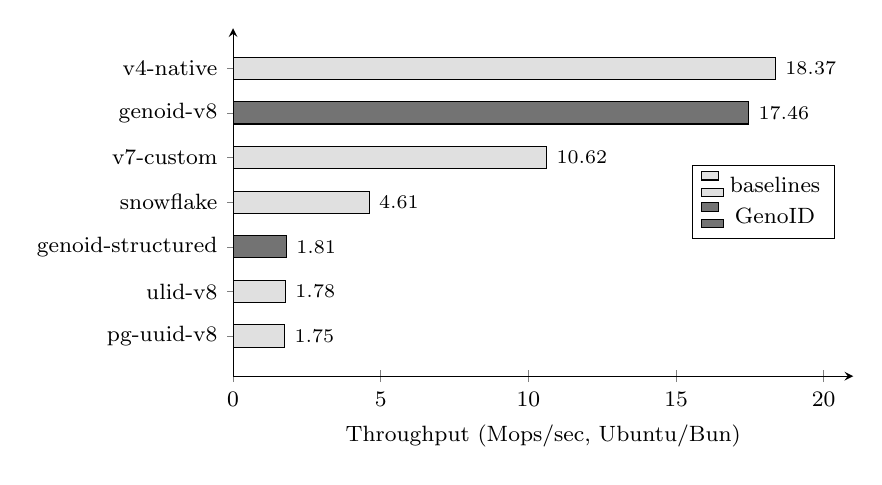
\begin{tikzpicture}
\begin{axis}[
  xbar, width=0.78\columnwidth, height=6cm,
  axis x line=bottom,
  axis y line=left,
  xmin=0, xmax=21,
  xlabel={Throughput (Mops/sec, Ubuntu/Bun)},
  symbolic y coords={pg-uuid-v8,ulid-v8,genoid-structured,snowflake,v7-custom,genoid-v8,v4-native},
  ytick={pg-uuid-v8,ulid-v8,genoid-structured,snowflake,v7-custom,genoid-v8,v4-native},
  nodes near coords, nodes near coords align={horizontal},
  every node near coord/.append style={font=\scriptsize},
  bar width=8pt,
  tick label style={font=\footnotesize},
  label style={font=\footnotesize},
  enlarge y limits=0.15,
  clip=false,
  legend style={font=\footnotesize,draw=black,at={(0.97,0.5)},anchor=east},
]
% baselines (light)
\addplot[xbar,bar shift=0pt,fill=black!12,draw=black] coordinates {
  (1.75,pg-uuid-v8) (1.78,ulid-v8) (4.61,snowflake) (10.62,v7-custom) (18.37,v4-native)};
% GenoID (dark)
\addplot[xbar,bar shift=0pt,fill=black!55,draw=black] coordinates {
  (1.81,genoid-structured) (17.46,genoid-v8)};
\legend{baselines, GenoID}
\end{axis}
\end{tikzpicture}%
}
\caption{Throughput by generator (Ubuntu/Bun, mean of 10 trials). The unstructured pooled variant (\texttt{genoid-v8}) nears native v4, isolating pooling cost; the structured \texttt{genoid-structured} runs at 1.81M ops/sec, matching \texttt{pg\_uuid\_v8} and \texttt{ulid-v8} while adding declarative multi-field composition.}
\label{fig:throughput}
\end{figure}

\begin{table}[!ht]
\caption{Throughput comparison (mean of 10 trials, Ubuntu/Bun; 95\% CI within $\pm$5\%).}
\label{tab:throughput}
\centering
\begin{tabular*}{\columnwidth}{@{\extracolsep{\fill}}lcc}

\hline\noalign{\smallskip}
\textbf{Generator} & \textbf{Ops/sec (Ubuntu, Bun)} & \textbf{NIST} \\
\noalign{\smallskip}\hline\noalign{\smallskip}
v4-native & 18.37M & -- \\
v7-custom & 10.62M & -- \\
genoid-v8 (pooled) & 17.46M & -- \\
pg\_uuid\_v8 & 1.75M & 15/15 \\
ulid-v8 & 1.78M & 15/15 \\
snowflake & 4.61M & -- \\
genoid-structured (dbkey) & 1.81M & 15/15 \\
\noalign{\smallskip}\hline

\end{tabular*}
\end{table}

Head-to-head against \texttt{pg\_uuid\_v8} ($n=2$M): both 0 collisions; uniformity 0.0051 vs 0.0066; \texttt{genoid-structured} matches or beats \texttt{pg\_uuid\_v8} on 5 of 7 runtime environments while adding declarative multi-field composition.

\subsection{Ablation: isolating pooling from composition cost}
\label{sec:ablation}
Two-parent pooled generation ($1.41$M ops/sec) outperforms single-parent ($0.88$M ops/sec) by $1.6\times$, due to a pre-computed string buffer enabled by the pooled architecture. Quality is identical across both paths: 0 collisions, 0 violations, uniformity deviation $0.0051$ vs $0.0052$. The result confirms the Section~\ref{sec:entropy} proof: composition on random-type fields is entropy-neutral.

\subsection{Additional deployability checks}
\label{sec:deployability}
Concurrent generation shows 0 cross-worker collisions. A SQLite B-tree test shows genoid-structured incurs no insert tax versus random inserts, while uuid\_v7 carries ~24.5\% overhead. A cross-browser Playwright test (Chromium, Firefox, WebKit) reports 0 errors and 0 collisions.

\subsection{Cross-language reproducibility}
\label{sec:cross-lang}

To turn the portability claim into a checkable artifact, the composition core was reimplemented in Rust and verified against golden vectors from the TypeScript reference. A xorshift128+ PRNG with fixed seed and fixed \texttt{Date.now()} produce 1000 UUIDs per layout across all three structured layouts, then diffed byte-for-byte against committed golden files. Zero mismatches across all $3\times1000=3000$ UUIDs confirms the algorithm is language-agnostic at the bit level.

The golden vectors caught two classes of porting bug (a byte-consumption mismatch in \texttt{eventsourcing}'s \texttt{node}-typed field and a missing seed-state reset) that a prose-only specification would have missed. The vectors are checked into \texttt{golden/} and verified in CI on every push, serving as an executable specification for any future port.

In production, each port draws from its own OS CSPRNG; the seeded byte stream exists only for cross-language verification. Different buffering in a Rust port would be no less correct for producing different byte sequences.

\section{Related Work}
\label{sec:related-work}
\subsection{UUID standards: RFC 4122 to RFC 9562}
UUIDs originated as RFC~4122 (versions~1--5), obsoleted by RFC~9562 (2024), which adds versions~6, 7, and~8~\cite{1}. UUIDv4 carries 122 CSPRNG bits but lacks order; UUIDv7 prepends a 48-bit timestamp for index locality~\cite[\S5.7]{1}; UUIDv8 is explicitly experimental, with the RFC providing no creation algorithm for its 122 bits~\cite[\S5.8]{1}.
\subsection{Sortable and structured identifiers}
RFC~9562 surveyed sixteen prior implementations~\cite{1}. Representative members: ULID~\cite{2} (48-bit timestamp + 80-bit randomness), KSUID~\cite{3} (32-bit timestamp + 128-bit randomness), Snowflake~\cite{4} (timestamp $|$ worker $|$ sequence), TypeID~\cite{5} (typed prefix over UUIDv7), and COMBGUID (embedded timestamp). Time-ordered identifiers improve database behavior~\cite{6}, with academic comparisons of UUIDv4/v7/ULID for distributed systems~\cite{8}. This is a well-explored field limited to fixed, hand-coded layouts; none offers a declarative framework for arbitrary multi-field v8 composition.
\subsection{Steganographic UUIDs: closest prior art}
\texttt{pg\_uuid\_v8}~\cite{7}, a PostgreSQL C extension (PGXN, May~2026), is the closest prior art. It generates v4-compliant UUIDs with an encrypted microsecond timestamp (XOR or AES), recoverable by extraction function. GenoID differs: \texttt{pg\_uuid\_v8} offers one fixed stego layout with no multi-field abstraction or repair, while GenoID provides a declarative, multi-field DSL and constraint-guided repair as a portable library.

On throughput, prior work amortizes CSPRNG draws via pooling~\cite{10}, and PostgreSQL~18 ships a native \texttt{uuidv7()}~\cite{11}; GenoID adopts the same principle with a 256-UUID pool.

\section{Threats to Validity}
\label{sec:validity}
We disclose these openly, ranked by expected reviewer pressure.

\textbf{External validity.} Rust reimplementation produces byte-identical output across 3000 seeded UUIDs and three layouts. Performance portability remains future work. Benchmarks run on shared CI runners; numbers are relative comparisons.

\textbf{Construct validity.} NIST PASS/FAIL is necessary but not sufficient for security; Section~\ref{sec:security} provides a threat model and entropy accounting.

\textbf{Internal validity.} Benchmark confounds are mitigated by mean $\pm$ SD over 10 trials with 95\% CI and Welch $t$-tests. Two implementation bugs (a byte-consumption mismatch in \texttt{eventsourcing}'s \texttt{node}-typed field and a missing seed-state reset) were caught by the test suite before publication. NIST runs unconditionally; dieharder is a CI-budget curation.

\textbf{Conclusion validity.} Throughput comparisons use Welch $t$-tests. ``0 collisions'' is reported alongside the birthday-bound expectation.



\section{Conclusion and Future Work}
RFC~9562 leaves version~8's 122 bits undefined; GenoID fills them with a declarative, portable algorithm. Its core contribution is the \texttt{V8Layout} abstraction: typed, constrained multi-field composition with a single shared repair pass, validated through formal proof, empirical testing across 100M identifiers, an adversarial security analysis, and a cross-language reproducibility check.

The highest-value next step is compiling a layout declaration into a specialized generator, replacing the generic field loop and repair dispatch with inlined, layout-specific code. This would push GenoID's throughput toward the pooled-CSPRNG floor while retaining the declarative interface, staking a clear path from framework to production primitive.

\begin{thebibliography}{00}

\bibitem{1}
K. Davis, B. Peabody, and P. Leach, ``Universally Unique IDentifiers (UUIDs),'' RFC 9562, Internet Engineering Task Force (IETF), May 2024.

\bibitem{2}
A. B. Peabody, ``ULID Specification.'' \url{https://github.com/ulid/spec}

\bibitem{3}
Segment, ``KSUID.'' \url{https://github.com/segmentio/ksuid}

\bibitem{4}
Twitter, ``Snowflake.'' \url{https://github.com/twitter-archive/snowflake}

\bibitem{5}
Jetify, ``TypeID.'' \url{https://github.com/jetify-com/typeid}

\bibitem{6}
J. Nilsson, ``The cost of GUIDs as primary keys,'' InformIT, 2002.

\bibitem{7}
ineron, ``pg\_uuid\_v8: PostgreSQL extension for steganographic UUIDs,'' May 2026. \url{https://github.com/ineron/pg_uuid_v8}

\bibitem{8}
N. Karimian Kakolaki, ``A comparative analysis of identifier schemes: UUIDv4, UUIDv7, and ULID for distributed systems,'' arXiv:2509.08969, Sep.~2025.

\bibitem{10}
pscheid92, ``uuid: Go implementation of RFC 9562 with V8 and pooled/batch APIs.'' \url{https://pkg.go.dev/github.com/pscheid92/uuid}

\bibitem{11}
PostgreSQL Global Development Group, ``UUID functions,'' PostgreSQL~18 Documentation. \url{https://www.postgresql.org/docs/current/functions-uuid.html}

\bibitem{12}
L. E. Bassham, A. L. Rukhin, J. Soto, J. R. Nechvatal, et al., ``A Statistical Test Suite for Random and Pseudorandom Number Generators for Cryptographic Applications,'' NIST SP~800-22 Rev.~1a, Apr.~2010.

\bibitem{13}
R. G. Brown, ``Dieharder: A Random Number Test Suite,'' Duke University, 2007. \url{https://webhome.phy.duke.edu/~rgb/General/dieharder.php}

\end{thebibliography}


\end{document}
